\documentclass[a4paper, 10.5pt, twoside]{jreport}

% include
\usepackage{gra_yasuda}
\usepackage{lscape}
\usepackage{graphicx}
\usepackage{here}
\usepackage{color}
\usepackage{amsmath}
\usepackage{subfig}
\usepackage{tascmac}
\usepackage{url}
\usepackage{ascmac}
\usepackage{booktabs}
\usepackage{otf}
\usepackage{comment}



%タイトル
\title{心理的効果を用いた人間とエージェントの繰り返し交渉戦略}
\etitle{Repetitive negotiation strategy of human and agent \\ using psychological effect}

%名前
\author{松下 昌悟}
\eauthor{Shogo MATSUSHITA}

%入学年度
\enteryear{2017}
%卒業年度
\graduateyear{2018}

%学籍番号
\studentnumber{17268508}

%提出日
\date{平成30年1月xx日}

\begin{document}

%ここで行ピッチを指定
%フォントを変えるとサイズがリセットされてしまうので注意
\setlength{\baselineskip}{8truemm}


%ここから内容

% Chapter 3
\chapter{繰り返し交渉戦略の提案}\label{cha:3}

\section{段階的要請法(Foot-in-the-Door technique)}
段階的要請法は交渉の際に用いられる心理的手法である.
段階的要請法の概要を図\ref{fig:foot}に示す.
段階的要請法では,最初に相手に対して小さい要求を行い,徐々に要求を上げていく手法である.
この手法は自分の行動を一貫したものにしたいという人間の一貫性の原理を利用した交渉術である.

図\ref{fig:foot}では売り手は買い手に対して話を聞いてもらうという小さな要求を行い,
次にこの要求を承諾した買い手に対して商品を購入してもらうという大きな要求を行なっている.
このように,段階的要請法では事前に小さな要求を相手に承諾させることで真の要求を相手に拒否させづらくさせることが可能である.

\begin{figure}[h]
  \centering
  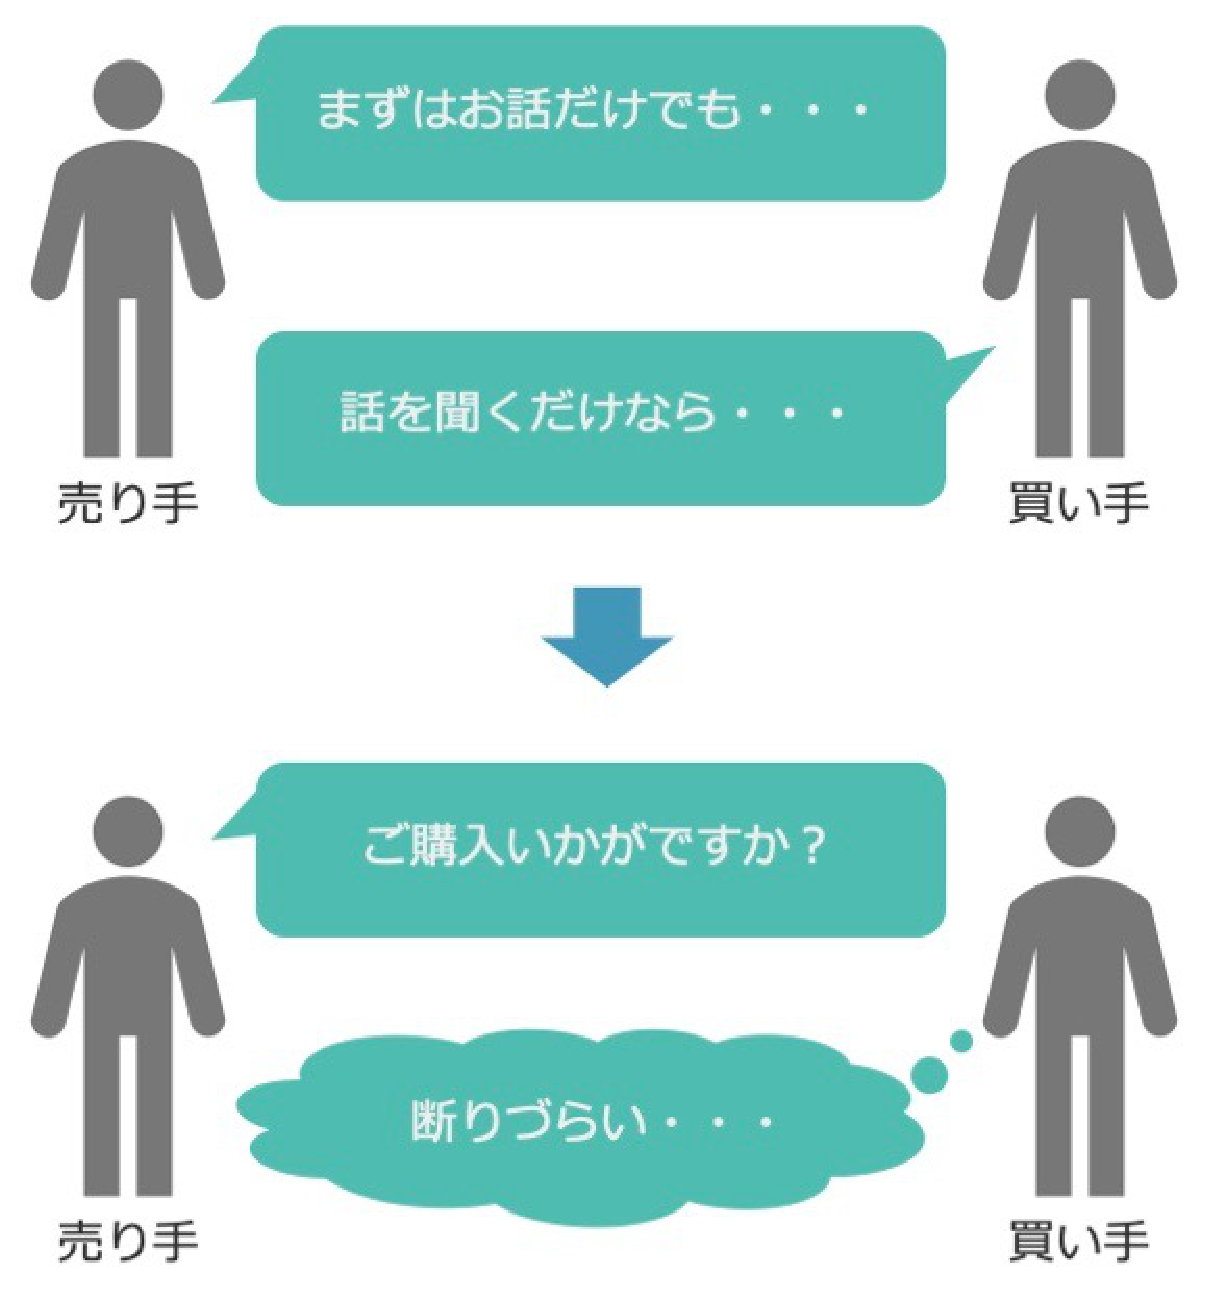
\includegraphics[width=10truecm]{image/foot.eps}
  \caption{段階的要請法の概要}
  \label{fig:foot}
\end{figure}

\section{譲歩的要請法(Door-in-the-Face technique)}

譲歩的要請法は交渉の際に用いられる心理的手法である.
譲歩的要請法の概要を図\ref{fig:door}に示す.
譲歩的要請法では,段階的要請法とは対照的に最初に相手に対して大きい要求を行い,徐々に要求を下げていく手法である.
この手法は相手が譲歩してきたため自分も譲歩した方が良いという人間の返報性の原理を利用した交渉術である.

図\ref{fig:door}では売り手は買い手に対して3万円で商品を買ってもらうという大きな要求を行い,
次にこの要求を拒否した買い手に対して商品を値下げし2万円で商品を買ってもらうという小さな要求を行なっている.
このように,譲歩的要請法では事前に大きな要求を行い,相手に要求を拒否させることで真の要求を相手に拒否させづらくさせることが可能である.

\begin{figure}[h]
  \centering
  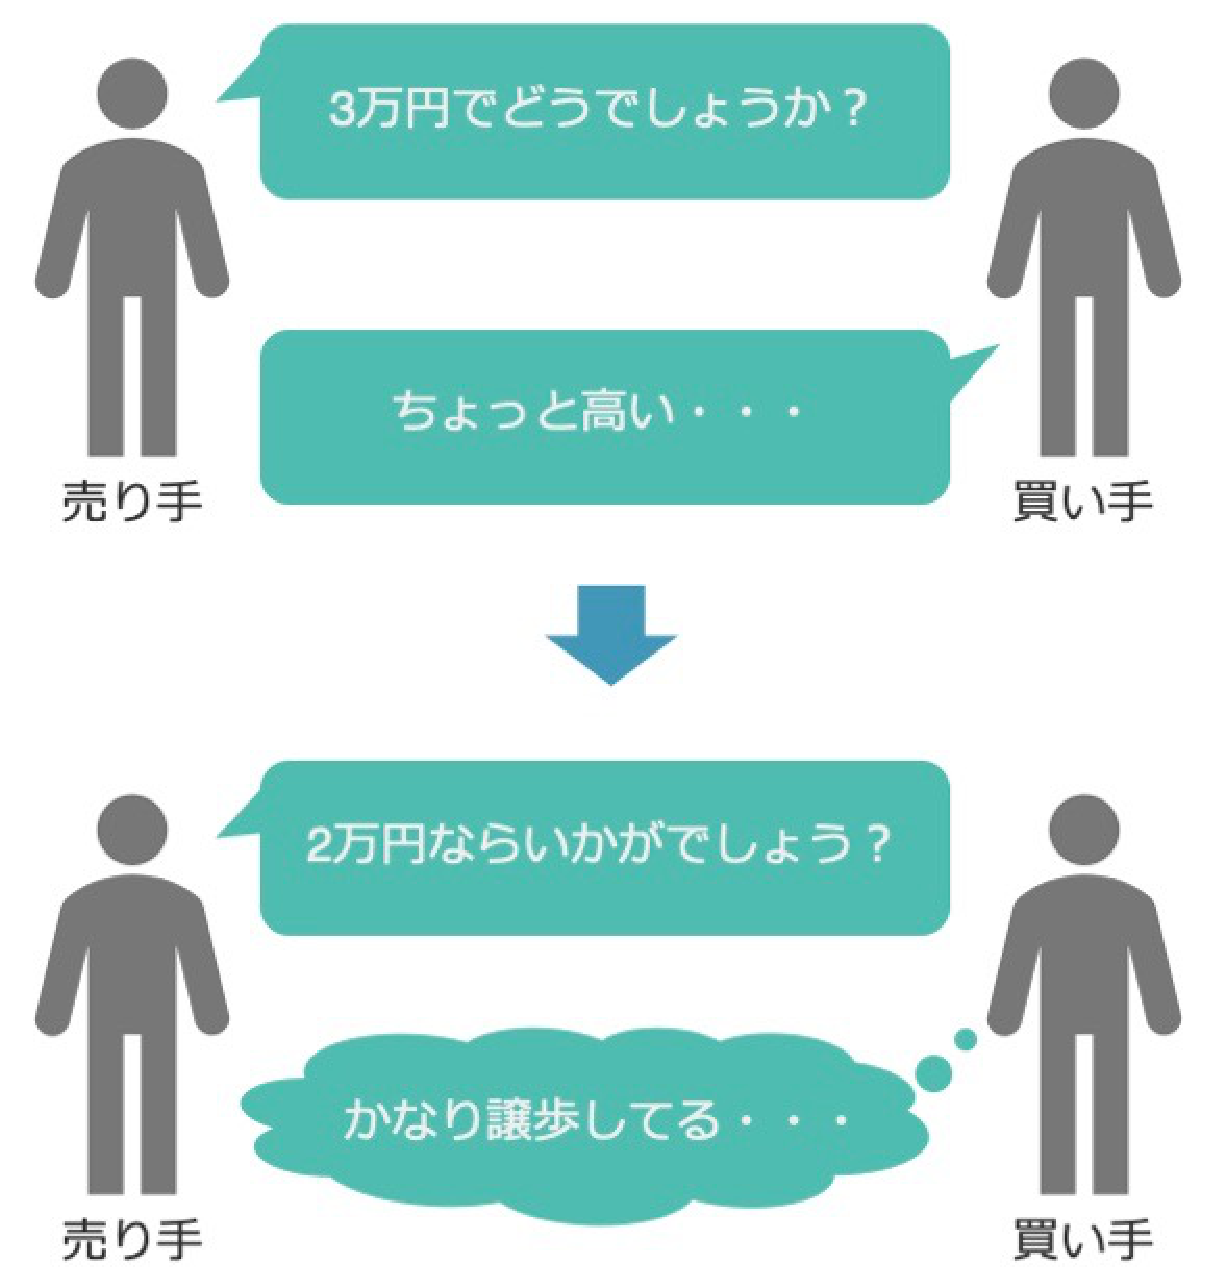
\includegraphics[width=10truecm]{image/door.eps}
  \caption{譲歩的要請法の概要}
  \label{fig:door}
\end{figure}

\section{段階的要請法と譲歩的要請法を組み合わせた交渉戦略の提案}

本稿では,先述した段階的要請法と譲歩的要請法を組み合わせることで繰り返し交渉に対応した戦略を提案する.
提案手法の概要を図\ref{fig:propose}に示す.

提案手法では相手の提案を受諾する水準を変化させる.1回の交渉ごとでは,時間経過に伴って水準を変化させる.
すなわち,図\ref{fig:propose}のように交渉開始時の水準が\mathrm{L}であった場合,時間経過によって水準を\mathrm{L\pm \alpha}に変化させる.以下,この水準を内側の水準と記述する.
また,同時に交渉回数の増加に伴って水準を変化させる.
すなわち,図\ref{fig:propose}のように1回目の交渉開始時の水準が\mathrm{L}であった場合,2回目の交渉開始時の水準を\mathrm{L\pm \meta}に変化させる.以下,この水準外側の水準と記述する.

\begin{figure}[h]
  \centering
  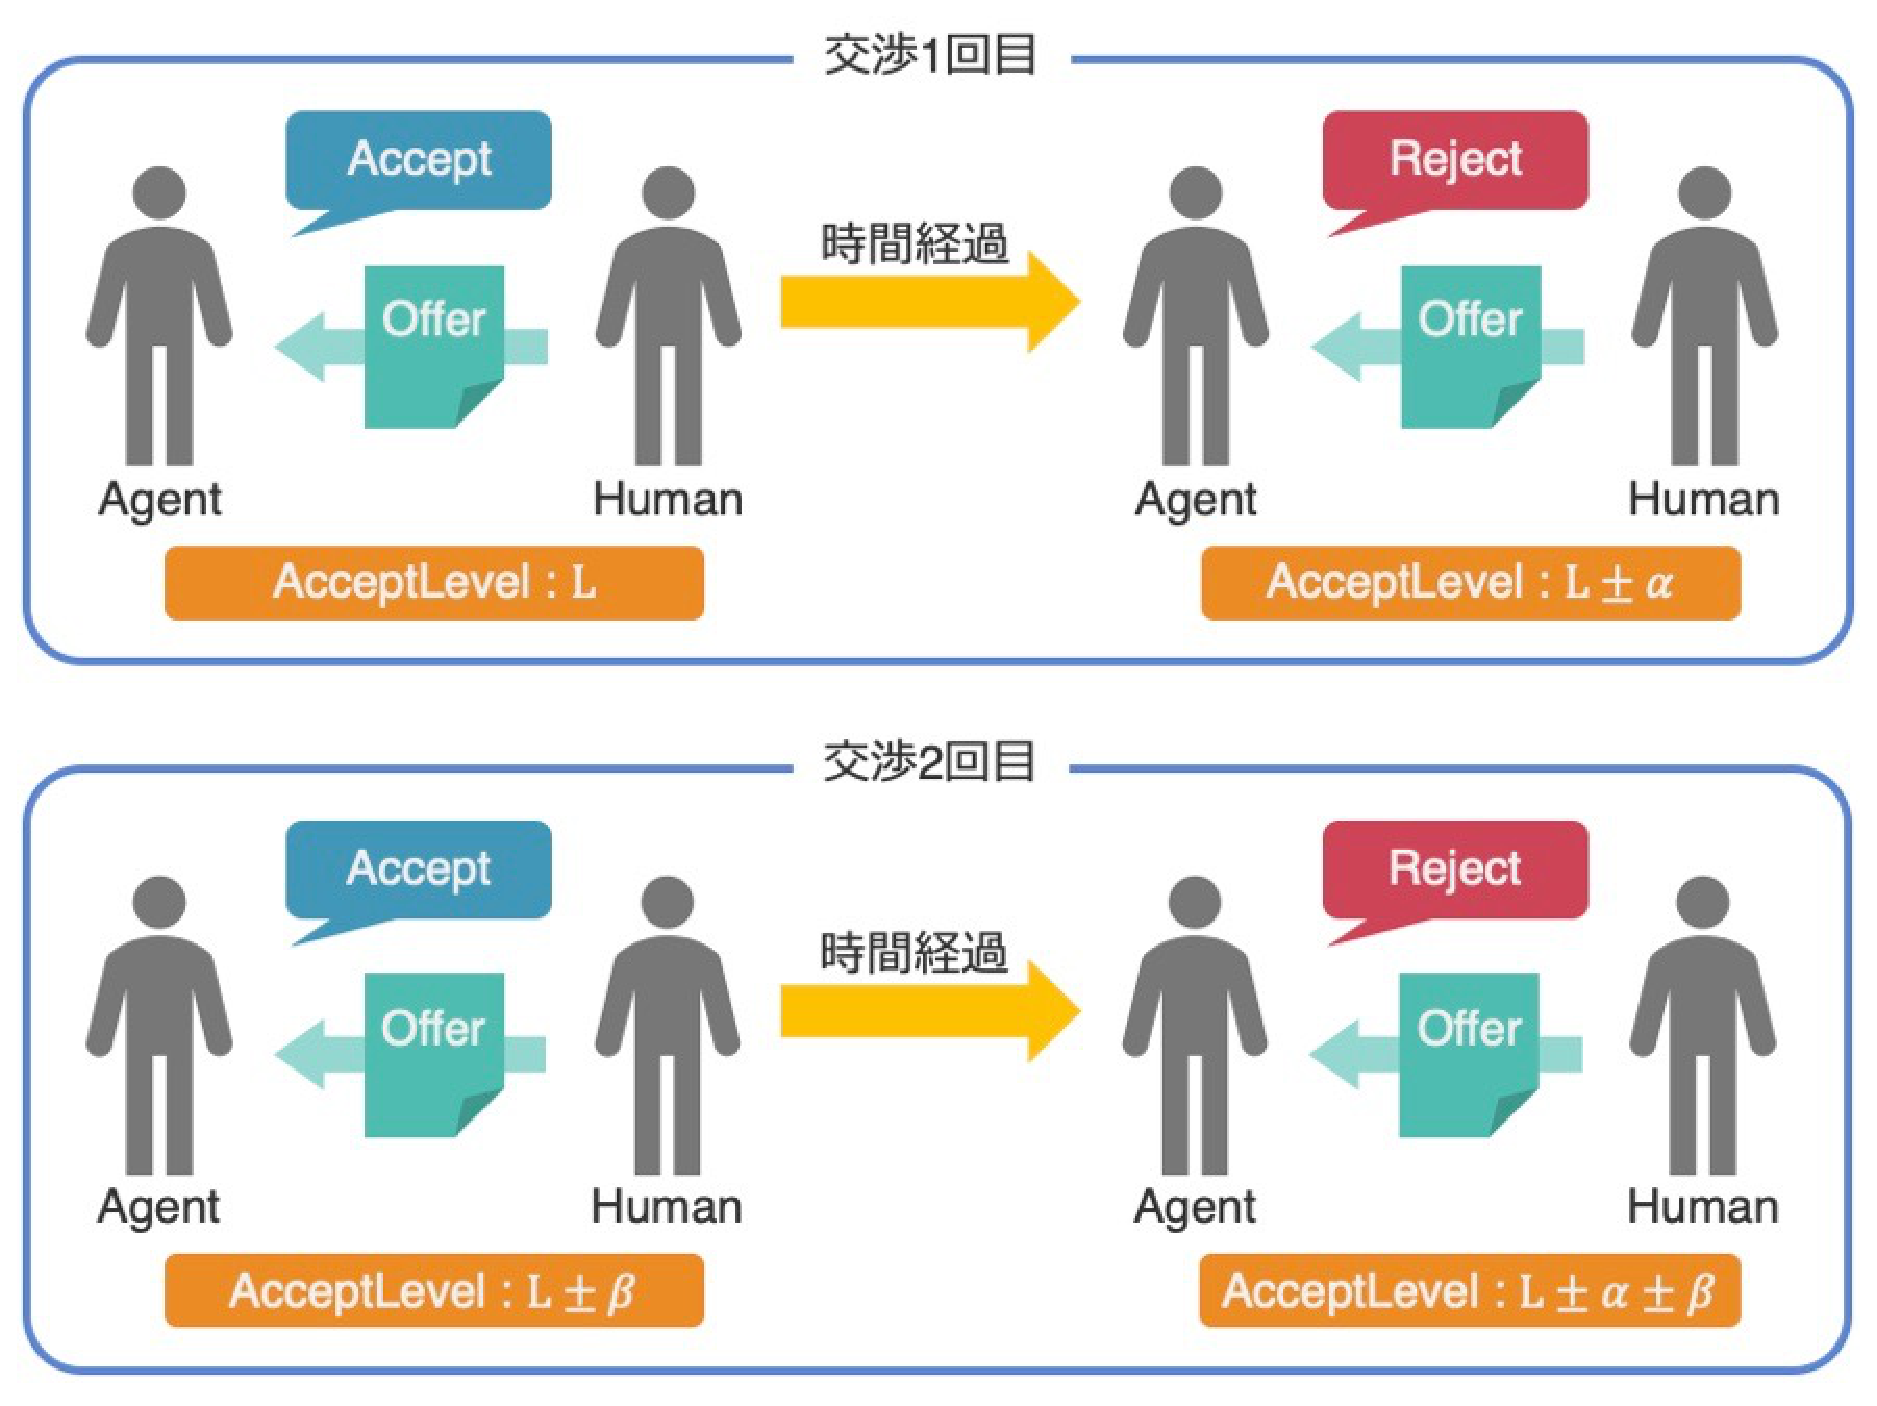
\includegraphics[width=15truecm]{image/propose.eps}
  \caption{提案手法の概要}
  \label{fig:propose}
\end{figure}

提案手法では,これら2種類の水準の変化を組み合わせることで,繰り返し交渉に対応する.
水準の変化にそれぞれ段階的要請法,譲歩的要請法,水準を変化させない方法の3種類を適用した9種類の戦略を用意する.
戦略の組み合わせと対応する戦略名を表\ref{tab:strategy}に示す.
表\ref{tab:strategy}の9種の戦略の内,内側および外側の戦略がどちらも変化しないNotNotはベースラインとして使用し,NotNotを除外した8種類の戦略を提案手法とし,第4章の予備実験および第5章の評価実験を行う.

\begin{table}[htb]
  \begin{center}
    \caption{戦略の組み合わせ}
    \label{tab:strategy}
    \begin{tabular}{|c|c|c|c|c|} \hline
      戦略名 & 内側の戦略 & 外側の戦略 & \alpha の値 & \beta の値 \\ \hline \hline
      NotNot & \multirow{3}{*}{なし} & なし & \multirow{3}{*}{0} & 0 \\ \cline{1-1} \cline{3-3} \cline{5-5}
      NotFoot & & 段階的要請法 & & $> 0$ \\ \cline{1-1} \cline{3-3} \cline{5-5}
      NotDoor & & 譲歩的要請法 & & $< 0$ \\ \hline
      FootNot & \multirow{3}{*}{段階的要請法} & なし & \multirow{3}{*}{$> 0$} & 0 \\ \cline{1-1} \cline{3-3} \cline{5-5}
      FootFoot & & 段階的要請法 & & $> 0$ \\ \cline{1-1} \cline{3-3} \cline{5-5}
      FootDoor & & 譲歩的要請法 & & $< 0$ \\ \hline
      DoorNot & \multirow{3}{*}{譲歩的要請法} & なし & \multirow{3}{*}{$< 0$} & 0 \\ \cline{1-1} \cline{3-3} \cline{5-5}
      DoorFoot & & 段階的要請法 & & $> 0$ \\ \cline{1-1} \cline{3-3} \cline{5-5}
      DoorDoor & & 譲歩的要請法 & & $< 0$ \\ \hline
    \end{tabular}
  \end{center}
\end{table}

%内容ここまで

\chapter*{謝辞}
本論文を執筆するにあたり,多数の方々からご指導・ご協力いただきましたことを,心より御礼申し上げます.

指導教員である藤田桂英准教授には,研究の機会を与えていただき,研究の方針に関する助言や発表練習等の
多大なるご指導や助言をいただきましたことを深く感謝いたします.

研究に関する知識のご教示に加えて,本実験の準備を行うにあたってWEBサーバを構築する際にお力添えいただいた松根鷹生様に深く感謝申し上げます.
また,藤田桂英研究室の皆様には研究に必要な知識や意見等をいただいたことを心より感謝いたします.

本実験を行うにあたってお忙しい中ご協力いただいた同期の編入生の方々,および安井貴規様がいなければ本論文は完成に至りませんでした.
心より御礼申し上げます.

最後に,様々な面で私を支えていただいた家族に,心より感謝いたします.ありがとうございました.

\bibliographystyle{plain}
\bibliography{reference}


\begin{comment}
%付録で発表論文をつけてアピールだ!!

\renewcommand{\bibname}{付録 発表論文一覧}
%\chapter{発表論文一覧}

\begin{thebibliography}{99}
\item S. Kakimoto and K. Fujita. 二者間複数論点交渉問題におけるパレートフロント推定手法の提案. Joint Agent Workshop and Symposium, 2014.
\item S. Kakimoto and K. Fujita. Estimating Pareto Fronts using Interdependency between Issues for Bilateral Multi-issue Closed Nonlinear Negotiations. Applications Knowledge and Service Technology for Life, Environment, and Sustainability workshop(KASTLES),2014.
\item S. Kakimoto and K. Fujita. 二者間非線形交渉問題におけるパレートフロント推定を利用した自動交渉エージェントの設計と評価. 情報処理学会 第177回 知能システム研究会, 2014.

\end{thebibliography}

\end{comment}

\end{document}

